\chapter{ERP: Enterprise resource planning}
Business systems known as enterprise resource planning (ERP) systems consolidate and simplify data from several organizational departments into a single, comprehensive solution that satisfies the demands of the whole corporation. ERP systems function by seamlessly integrating and coordinating activities and tasks that were previously fragmented and supported by older, stand-alone, and separate legacy systems.
The basis of an ERP system is a well-structured database that supports the operational and decision-making requirements of end users across the company and generates information for external constituencies, such as regulatory agencies and investors.
\begin{figure}\centering
    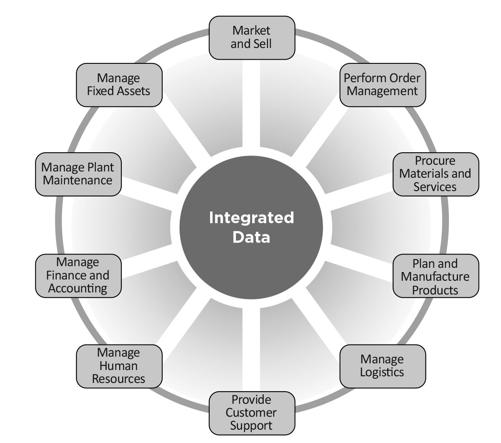
\includegraphics[scale=0.5]{Pictures/2_ERP_Processes.jpg}
    \caption{ERP-Supported Business Processes}
    \label{fig:2_ERP_Processes}
\end{figure}
\\
ERP systems are regarded as \textbf{cross-functional} in nature, since they satisfy the information needs of all end users, and also \textbf{process-centered} because they offer a clear, full, logical, and precise view of the business processes of the firm, which are groups of interconnected tasks that bring value to the enterprise.
Business operations frequently cross departmental boundaries and, in many circumstances, cross organizational boundaries, sharing data and information with external business partners like clients and suppliers, making ERPs essential within a company.
Some key business processes incorporated in ERP systems are shown in Figure \ref{fig:2_ERP_Processes}.

\section{Reasons for Implementing ERP}
Businesses that use ERP systems the most often have a lot of the same issues and frustrations. Figure \ref{fig:2_ERP_Reasons} lists the primary justifications for ERP adoption by businesses. A few of these reasons are explored below.

\begin{figure}
    \centering
    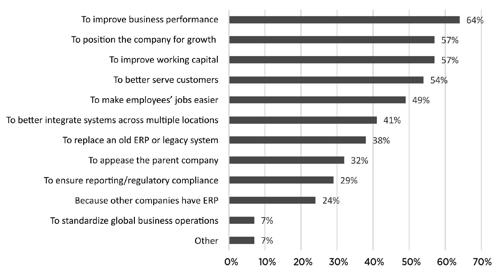
\includegraphics[scale=0.75]{Pictures/2_ERP_Reasons.jpg}
    \caption{Reasons for Implementing ERP}
    \label{fig:2_ERP_Reasons}
\end{figure}

\subsubsection{Improve business performance}
ERP improves business performance through the numerous best practices embedded within the several business processes. A \textbf{best practice} is a business procedure that is generally regarded as being more successful and/or efficient than others in a certain sector.
Companies that implement ERP will end up redesigning their previously disjointed, erroneous, slow, and ineffective processes to align with best practices in the software and can decrease operational costs, such as lower inventory costs, production costs, or purchasing costs, and increase revenue-generating processes, such as time to market, marketing and sales, and customer service.\\
Each view of best practices distinguishes one ERP vendor’s software from another’s, thus finding which ERP system's best practices match a buyer's demands is essential when choosing an ERP vendor's product since this fit influences the implementation's final success.
In order to find best practices across different industries and implement them into their solutions, the suppliers fund significant research and development (R\&D) initiatives. Additionally, it enables an ERP provider to provide niche versions of its software known as \textbf{vertical solutions}, which are essential due to the unique characteristics that each industrial sector has.

\subsubsection{Desire for growth}
Examples of growth strategies include market expansion and penetration, product diversification, and mergers and acquisitions (M\&A).
ERP systems help with market expansion through demand forecasting, which generates predictions to estimate the future requirements for items.
Advanced rule-based pricing is another feature of ERP software. This capability enables businesses to comprehend the present patterns and trends of the sector, consumers, and rivals before making any pricing modifications.
Businesses may expand their product lines and provide new items and features to their clients by diversifying their product offerings. Data on which items are selling and to whom may be found in ERP systems, as well as information on which products are just taking up space on the shelves.
Finally, an ERP may assist in standardizing procedures across organizations during an M\&A activity in order to integrate them into a common platform.

\subsubsection{Facilitate employees' work}
ERP systems are also recognized to make the duties of employees easier. ERP does this in part by providing employees with real-time access to information; this feature significantly enhances operations, corporate governance, and enterprise risk management, resulting in a horizontally "connected up," process-centered organization. ERP systems also offer an unified user interface and tool set that improves accuracy, encourages collaboration, and reduces misunderstanding. Finally, ERP systems empower users by providing them with access to data that was previously impossible to get due to fragmented procedures supported by many older systems.

\subsubsection{Lack of compliance}
Government and institutional compliance requirements continue to grow and evolve. Navigating through numerous legal, regulatory, and supply chain mandates has never been tougher. ERP systems can help companies comply with these requirements, such as GDPR, SOX or Food and Drug Administration.

\subsubsection{Data integration}
With ERP systems, data is better integrated since it is only gathered once and then shared throughout the company, reducing the risk of inaccuracies and duplications and eliminating time-consuming data checking, and reconciliation across systems. Because all users have access to up-to-date, accurate, and comprehensive data, this feature is advantageous to all of them. With ERP, since data is now kept in a single data repository, the process of fixing errors is made simpler because they only need to be fixed once.
Processes are also better integrated because they are managed within one system, not spread across multiple systems that have been cobbled together. When a corporation's systems are patched together from several sources, the scenario can cause problems on the operations designed to keep the organization functioning efficiently.

\subsubsection{Replacement an old ERP}
Having multiple disparate systems or operating an out-of-date ERP system, that runs on obsolete technology or that cannot support a company’s business processes, creates an IT maintenance nightmare. These systems may be complicated to customize, and installing fixes and upgrades can take up valuable time and resources. Additionally, because the vendor could no longer be in operation, it might not be viable to upgrade these systems.

\section{Disadvantages of ERP Systems}
An ERP system implementation is significantly more involved than merely installing commercially available software; it is a labor-intensive process that requires a variety of different tasks and, if managed incorrectly, might lead to the project's failure.
Companies shouldn't take the choice to deploy an ERP system lightly due of its importance. All workers, from functional users to IT professionals to top management, must be aware of the goals of the ERP project and collaborate to make the deployment successful.
Companies that are thinking about implementing an ERP system should perform due diligence in selecting the solution that best fits their needs and collaborating with experts who can help with different implementation-related tasks.

\subsubsection{People issues}
Top management can be a major problem if they do not establish a convincing “tone at the top” that the ERP system is a priority or if they don’t allocate adequate resources to its deployment.
Lack of support from the employees may also be a concern. The legacy systems that employees have used for years may make them feel quite at ease. They could oppose to the additional training, organizational adjustments, and modifications to business processes that are unavoidable, or they can claim that the system is too challenging, constrictive, or inflexible.
Employees who are resistant to the ERP system may create unproductive workarounds or create their own "shadow IT," such as spreadsheets or old systems, as a result of which they fail to use the system as intended.

\subsubsection{Software issues}
Because ERP systems are sophisticated and intricate, installing them sometimes necessitates paying high-priced system integrators. Companies frequently struggle to take control of technology and to use it to transform business processes in a quantifiable and sustainable way. A level of complexity that has not before been encountered and is difficult to absorb may also be added by the various capabilities, options, and setup requirements for businesses with relatively straightforward business requirements.

\subsubsection{Price tag}
ERP system deployments can cost millions of dollars and take years to complete, especially for big, international businesses. Additionally, once established, the ERP system requires ongoing "care and feeding" to keep it current, stable, and compatible with a variety of constantly evolving software programs with which it may interact. Companies often update and do larger improvements to the ERP system. This component of ERP might wind up costing more overall than the initial software licensing and implementation fees combined since maintenance charges are required annually.

\subsubsection{Standardization}
The above noted benefit of business process standardization may also be a drawback if the rigidity is inconsistent with the firm's culture or expectations. Additionally, a problem that must be resolved for the ERP installation to be effective is that the current corporate culture may not promote information exchange among business units or divisions. Vendors and system integrators actively advise businesses to adopt the best practices for ERP systems rather than customizing the software to fit their unique workflows. An exception, though, would be if businesses customized the software in accordance with a special business strategy that set them apart from rivals. The general guideline is that customizing the ERP software to get this capability is necessary if a certain procedure makes a business competitive or is required for compliance with a legislation.

\section{Modules}
ERP systems are offered as modules, which are collections of connected software applications that handle key organizational tasks like accounting or production. Each module is designed to support a particular business process.
The main modules, that provide basic functionalities for managing business processes, make up the \textbf{Core of the ERP}. This includes financial management, supply chain, human resources, customer relationship management, and other critical business processes. The "core" is the central and fundamental part of the ERP system and provides an integrated solution for managing company data.
Here are some of the most common modules found in ERP systems:
\begin{itemize}
    \item \textbf{Financial Management}: This module is responsible for managing financial transactions, such as accounts payable and receivable, general ledger, and financial reporting.
    \item \textbf{Accounting}: This module includes sub-modules for cost accounting, payroll, fixed asset management, and other accounting functions.
    \item \textbf{Human Resources}: This module manages employee information, benefits, payroll, and other HR functions.
    \item \textbf{Procurement}: This module covers all aspects of procurement, including vendor management, purchase order creation and management, and inventory management.
    \item \textbf{Supply Chain Management}: This module manages the flow of goods and services, including procurement, production, and logistics.
    \item \textbf{Production}: This module helps manage the production process, including planning, scheduling, and tracking.
    \item \textbf{Sales and Marketing}: This module supports sales and marketing activities, including lead management, opportunity tracking, and customer relationship management.
    \item \textbf{Customer Relationship Management (CRM)}: This module supports customer-facing activities, such as marketing, sales, and customer service.
\end{itemize}
The specific modules included in a particular ERP system can vary based on the size of the
organization and its unique business requirements. Most ERP software is flexible enough to allow
businesses to purchase only the components they require “a la carte”, this allows companies to have
a solution “tailor-made” to its needs. Modular architecture has the advantage of enabling ERP
suppliers to create product solutions for specific industries. Sometimes modules that support a
major business area are called a \textbf{suite} which comprises multiple sub-modules, or components.
An example is shown in Figure \ref{fig:3_ERP_Modules}, where ERP modules for a manufacturing company
are depicted.
\begin{figure}
    \centering
    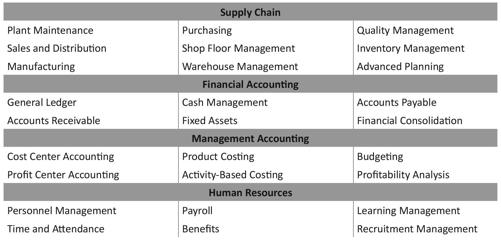
\includegraphics[scale=0.75]{Pictures/3_ERP_Modules.jpg}
    \caption{Examples of ERP Modules for a manufacturing company}
    \label{fig:3_ERP_Modules}
\end{figure}
\\
In summary, the various modules in an ERP system work together to provide a comprehensive solution
for managing business processes and data. By integrating all business functions into a single
system, organizations can streamline processes, reduce data duplication, improve business analytics,
and make more informed decisions.

\section{Technology}
An ERP system has a far-reaching impact that affects users across an entire organization, as well as
its customers, suppliers, and other business partners. With the need to support a large number of
users who have different processing and reporting requirements, it is important to have advanced and
adaptable software that utilizes cutting-edge technology. Given that the ERP system plays a crucial
role in fulfilling an organization's operational and information needs, it is essential to have a
thorough understanding of the technology that supports the integrated system, and provide a robust,
scalable, and user-friendly solution for managing a wide range of business processes and data.

\subsection{Three-Tier Client-Server Architecture}
The client-server architecture\textsuperscript{\cite{web_application}} is widely used in modern
computing, and is a fundamental aspect of many systems, including ERP systems. This architecture is
a computing model in which a server (\textbf{Back-end application}) provides services to clients
(\textbf{Front-end application}) over a network. The client requests a service or resource from the
server, and the server responds by providing the requested information or performing the requested
task. This architecture allows for efficient and scalable distribution of resources and tasks, as
the server can handle requests from multiple clients simultaneously.
\newline\newline
In this context we can separate an application into three logical components \textbf{(3-Tier
    architecture)}, which are the client tier, the application tier, and the database tier. This
architecture provides a scalable, flexible, and secure solution for software applications. In Figure
\ref{fig:2_ERP_arch} is showed a detailed explanation of each tier.

\begin{figure}\centering
    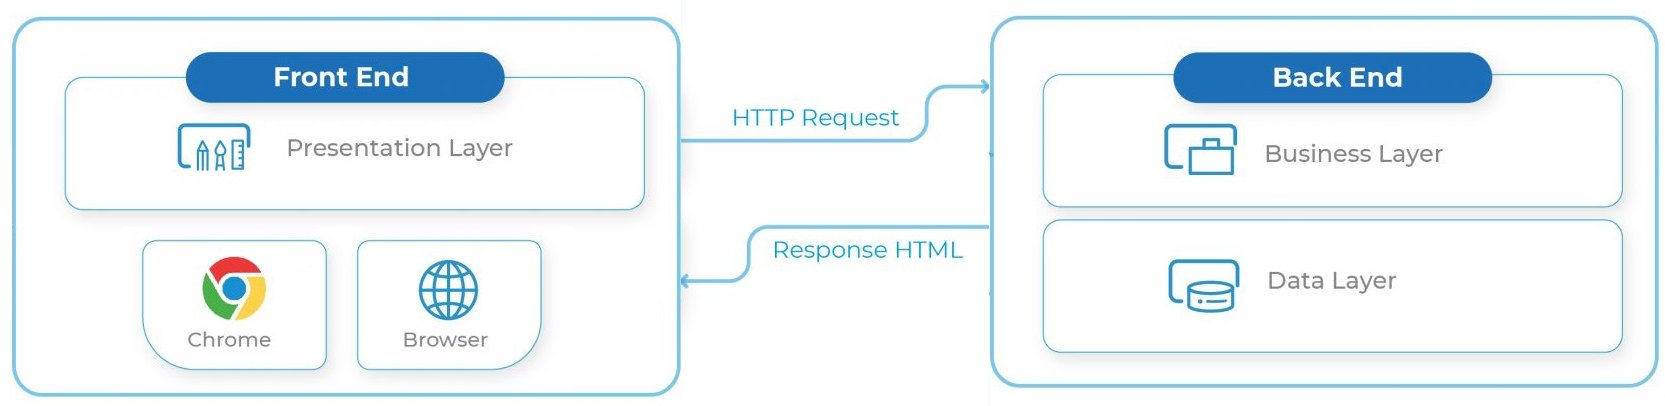
\includegraphics[scale=0.33]{Pictures/2_ERP_arch.jpg}
    \caption{Web Application Architecture}
    \label{fig:2_ERP_arch}
\end{figure}

\begin{itemize}
    \item \textbf{Client Tier - Presentation layer}: This tier is responsible for presenting the user interface to the end-user. It provides the interface through which users interact with the application. The client tier can be implemented as a standalone application or as a web application accessed through a web browser.
    \item \textbf{Application Tier - Business layer}: This tier is responsible for processing the user requests and returning the results to the client tier. It is responsible for handling the business logic and data processing. The application server tier is typically implemented as a web server.
    \item \textbf{Database Tier - Data access layer}: This tier is responsible for storing and managing the vast amount of data generated by the application. It is a key component of a web application that stores and manages information for a web app. You can search, filter and sort information based on user request. It is typically implemented using a robust database management system.
\end{itemize}
The three-tier architecture allows for a separation of concerns, with each tier having a specific role and responsibility. This separation makes it easier to develop, maintain, and upgrade the application, as changes can be made to one tier without affecting the others. Additionally, by dividing the system into separate tiers, the performance and security are improved. The client does not have direct access to the data, instead, all data passes through the application server which controls and regulates access to the information. This allows for more efficient and secure management of data. The ability to deploy application servers on multiple machines provides higher scalability, better performance and better re-use. \\
The Three-Tier Client-Server Architecture is a widely used architecture for ERP systems, as it provides a scalable, flexible, and secure platform for managing complex business processes and data.


\subsection{Deployment}
An ERP system can be deployed in two ways: On-premise or on Cloud, each with its own advantages and disadvantages. The best deployment method depends on the specific needs and requirements of the organization.

\subsubsection{On-Premise}
The conventional approach to ERP deployment is \textbf{on-premise ERP}.
In this deployment method, the ERP software is installed and run on computers within an organization's own physical facilities. This allows for complete control over the software and data, but also requires the organization to provide the necessary hardware, storage, and technical support. Companies choosing the “on-prem” option are usually larger companies with bigger budgets, an existing IT infrastructure in place, and knowledgeable IT personnel to support the software and infrastructure. Due to the large upfront cost required, which often includes the cost of both hardware and software, on-premise ERP is typically seen as a capital investment.

\subsubsection{Cloud}
\textbf{Cloud ERP} deployment is becoming increasingly popular, where the ERP system is hosted by a vendor or third party on shared computing resources that can be accessed through the internet. These resources are maintained in data centers dedicated to hosting various applications on multiple platforms.
This deployment method offers more scalability and flexibility, as well as reduced hardware and technical support expenses, but it requires an organization to have trust in a third party with access to its data.
Customers have access to the ERP system as needed and pay for the software on a monthly or yearly basis. This method of paying for ERP software on a subscription basis is called \textbf{software as a service (SaaS)}, an attractive option for businesses looking to reduce upfront expenses and to budget for ERP long-term.
Nowadays, nearly all ERP vendors offer some form of cloud deployment because it has many advantages compared to on-premise deployment.

\subsubsection{Advantage}
\begin{itemize}
    \item One key advantage is that ERP cloud providers maintain, upgrades and handle maintenance for the infrastructure of the ERP system.
    \item Cloud ERP is more scalable than on-premise, which is ideal for startups and fast-growing businesses.
    \item Companies that choose cloud ERP over on-premise can now enjoy more peace of mind that the cloud provider has up-to-date controls in place such as data backup, dual factor authentication, encryption for confidential data, and a disaster recovery plan.
\end{itemize}

\subsubsection{Disadvantages}
\begin{itemize}
    \item Many vendors offering cloud solutions are primarily focused on just one particular area. Very few cloud providers are offering a suite of products to meet the needs of medium-to-large organizations.
    \item Many cloud ERP solutions are limited in what the customer can do in terms of customization.
    \item Although cloud ERP is generally thought to be less expensive than on-premise, research has shown that over a 10-year window, the total costs for each converge. While expenses for cloud ERP are less upfront than on-premise, the costs catch up over time. Thus, the costeffectiveness of cloud ERP is not as great as initially thought.
\end{itemize}

\subsection{Customization}
It's uncommon for an ERP system to fully meet a company's needs, especially if the company is a large, global organization. There are often problems that go beyond what the ERP software can accommodate through configuration. Examples of these issues include:
\begin{itemize}
    \item Creating additional functionality not provided by the ERP system \item Establishing connections between the ERP system and third-party systems
    \item Adding extra fields to the ERP database
\end{itemize}
These types of problems usually require development and programming to enhance the ERP system. This is known as customization, which involves adding custom code to increase the capabilities and features of the ERP system. Customization is typically performed when all efforts to find a solution through configuration have failed. As customization requires time and money, companies should aim to minimize it.

\section{Market}
The ERP market is estimated at \$43.72 billion in 2020, and is projected to reach \$117.09 billion
by 2030, at a compounded annual growth rate of 10.0\%\textsuperscript{\cite{erp_market}}. The increase in the ERP market can be
attributed to the growing interest from small and medium-sized businesses and the development of new
ERP applications for both cloud and mobile platforms. However, not all ERP vendors offer the same
quality of software, which can be divided into three categories based on specific criteria, as
presented in a table \ref{tab:table_ERP_Tiers}.
\begin{itemize}
    \item \textbf{Tier I} (Enterprise Class) is software designed for large, worldwide corporations with significant market capitalization and annual revenues that exceed \$750 million. These solutions are very costly due to their extensive capabilities, including the ability to manage complex organizational structures and address international concerns, like multiple currencies and varying accounting regulations. Only a few ERP vendors have the necessary size, resources, and comprehensive functionality to support the high volume of daily transactions that Tier I companies typically encounter.
    \item \textbf{Tier II} (the Mid-Market Class) category of ERP systems is intended for medium-sized companies and can be further divided into upper and lower sub-categories. Upper Tier II systems are for companies with annual revenues ranging from \$250 million to \$750 million. Lower Tier II systems typically are for companies with annual revenues between \$10 million and \$250 million.
          These vendors offer software that is designed for either single or multiple legal entities and locations, but with limited functionalities compared to Tier I vendor solutions. As a result, these ERP systems are less expensive than Tier I systems. Typically, they are easier to implement and support and are designed specifically for only a few industries.
    \item \textbf{Tier III} (Small Business Class) ERP systems are made for smaller businesses with annual revenue below \$10 million, operating within a single country. They are the most affordable among the different tiers of ERP systems. The market is saturated with many software providers in this category, some of which offer robust point solutions that can be utilized to enhance a Tier I or Tier II ERP system.
\end{itemize}
\begin{table}
    \centering
    \begin{tabular}{p{4.4cm} | p{4.4cm} | p{4.4cm}}
        \hline\hline
        Tier I                       & Tier II                          & Tier III                              \\
        \hline
        %\hspace*{1.3em}
        High complexity              & Medium complexity                & Low complexity                        \\
        Highest cost                 & Medium cost                      & Lowest cost                           \\
        Many industry solutions      & Fewer industry solutions         & Fewest industry solutions             \\
        Large companies              & Mid-market companies             & Small companies                       \\
        Support global functionality & Operate in more than one country & Does not support global functionality \\
        \hline \hline
    \end{tabular}
    \caption{Characteristics of ERP Vendor Tiers}
    \label{tab:table_ERP_Tiers}
\end{table}
The ERP market is experiencing a trend where Tier II and Tier III vendors are aiming to serve larger companies by improving their software's capabilities and scalability, while Tier I vendors are reaching smaller companies by offering simplified versions of their software and acquiring cloud vendors. This is causing the boundaries between ERP tiers to become less distinct as vendors strive to increase their market share.
Table \ref{tab:table_ERP_vendor} presents some example of ERP systems in  tiers.
\begin{table}
    \centering
    \begin{tabular}{p{4.4cm} | p{4.4cm} | p{4.4cm}}
        \hline\hline
        Tier I      & Tier II                 & Tier III \\
        \hline
        SAP S4/HANA & Microsoft Dynamics 365  & Sage     \\
        Oracle EBS  & NetSuite                & Aptean   \\
        Infor LN    & SAP Business All-in-One & ASC      \\
        Infor M3    & ODOO                    & ECI      \\
        \hline \hline
    \end{tabular}
    \caption{Example ERP Vendors in Tiers}
    \label{tab:table_ERP_vendor}
\end{table}

\subsection{Cost}
%articolo "Be Wary of the Economics of Serverless Cloud Computing"
%documento pricing guide BC
Numerous ERP projects run over budget, often as a result of unanticipated organizational or
technological problems, scope expansion, or an unrealistic project budget. Budgeting for ERP can be
difficult since some costs are difficult to predict at first. This section will go into depth about
every expense that goes into calculating the system's total cost of ownership \textbf{total cost of
    ownership (TCO)}. Some of these costs will be one-time costs, while others will be
recurring\textsuperscript{\cite{erp}}.

\subsubsection{Software License Costs}
Typically, an ERP system’s price tag depends on the:
\begin{itemize}
    \item Number of employees that will be using the system
    \item Vendor tier being deployed, Tier 1 software is more expensive than Tier 2, while Tier 3 would be the least expensive
    \item Number of modules purchased
\end{itemize}
The vast majority of ERP software licenses are supplied using a \textbf{perpetual licensing model}, which requires paying an upfront licensing price before the vendor grants access to the program for an endless amount of time. Additionally, customers must pay annual maintenance costs in order to get support, updates, and future software upgrades. For on-premise implementations, perpetual licensing is standard. With perpetual licensing, a couple of license methods are used:
\begin{itemize}
    \item \textbf{Named user licensing}. A company determines how many unique users will use the ERP system and pays a licensing charge for each of them. Numerous ERP vendors provide different named user categories, such as heavy user licensing, for users who utilize more system capability and are thus paid a larger license fee, or casual user licensing, for users who just read reports or lists.
    \item \textbf{Concurrent user licensing}. A perpetual license type enables an unlimited number of designated users and accounts, but restricts the number of individuals who can actively use the software at one time. Concurrent user licensing is often cheaper than named user licensing as it only requires payment for the estimated number of simultaneous users. However, it's essential to accurately predict the number of concurrent users, otherwise, employees may experience difficulties logging on and using the software.
\end{itemize}

\subsubsection{Third-Party Software License Costs}
In some cases, a company has specific requirements that cannot be fulfilled by the ERP system they have purchased, and modifying the ERP to meet those requirements is too costly. To address this, third-party software known as "bolt-ons" can be used. These provide additional functionality or logic to help solve specific business needs. To ensure seamless integration with the ERP system, it is advisable to get recommendations from the ERP vendor or system integrator on which bolt-on solution will work best.

\subsubsection{Hardware and IT Infrastructure Costs}
The implementation of an ERP system requires a strong and up-to-date IT setup. If the ERP is run on-site, a company will need to invest in IT hardware such as servers, routers, backup, storage devices, desktops, laptops, tablets, and printers. They will also need to consider measures for failover, network access, power supply, and security. This may involve hiring additional staff and increasing data center space, with costs ranging from one-time expenses like purchasing servers to ongoing expenses like utility bills and salaries.

\subsubsection{Database License Costs}
The cost of the database in an ERP project can range from a few thousand dollars to hundreds of thousands of dollars, depending on several factors such as the type of database, the size of the data being stored, and the number of users accessing the database. ERP vendors will provide the specifications for the type of database needed.

\subsubsection{Implementation Costs}
The expenses related to the implementation of ERP software are among the most pricey parts of the total cost of ownership (TCO). The cost of functional and technical consultants, who play a key role in the implementation, can be a major part of these expenses, depending on how much a company is going to rely on the system integrator.
The complexity of the project and consultants from different geographical locations may also affect the hourly rate charged.

\subsubsection{Maintenance and Support Costs}
The cost of an ERP system doesn't end once the software is up and running. To ensure the system continues to run smoothly, companies need to have a plan for ongoing maintenance and support, also known as \textbf{application management services (AMS)}. This includes functional and technical support, updating and patching, monitoring the software, and backup and recovery. Some companies can handle these tasks in-house, while others may hire a third-party company to provide these services. The cost of maintenance typically ranges from 18\% to 25\% of the original software license cost and can be paid directly to the ERP vendor or to the third-party company managing the system. \\
For software support, various levels are available, with the higher levels offering more services at a higher cost. Premium support could include having a representative from the ERP vendor on-site during the project implementation and for a period of time post-implementation, as well as prioritized access to help tickets. Basic support might only provide access to a help portal where customers can log tickets and get answers to questions.

\subsubsection{Cloud}
The Total Cost of Ownership (TCO) in a cloud context is the same as what we previously discussed,
but often, all of the costs are included in a single \textbf{subscription-based licensing}.
Customers subscribing to this model are granted program access for a set duration, such as monthly
or annually, which covers not only the use of the software but also maintenance, support, scheduled
updates, and upgrades provided by the cloud vendor. This comprehensive subscription often includes a
basic database offering, with the flexibility to expand storage for an additional fee.
\newline\newline
Predominantly, ERP applications are marketed as \textbf{Software as a Service (SaaS)}, a cloud-based
delivery model wherein the vendor shoulders the responsibility for the underlying infrastructure,
including hosting, maintenance, and support. This implies that the costs for IT infrastructure, when
the ERP system is hosted by the vendor or a third-party provider, are bundled into the monthly
subscription fee. Companies utilizing public cloud platforms like Microsoft Azure would typically
pay a recurring fee for the infrastructure lease in addition to the software licensing fees due to
the ERP vendor.

\subsection{Competitors}
The ERP (Enterprise Resource Planning) market is experiencing a significant shift with the emergence
of smaller, more agile players. These smaller vendors are challenging the traditional dominance of
larger, established companies like SAP, Oracle, and Microsoft. Characterized by their innovative,
cloud-native solutions, these emerging players focus on delivering specialized and industry-specific
ERP systems. This approach contrasts with the one-size-fits-all, monolithic systems traditionally
offered by the larger vendors\textsuperscript{\cite{erp_competitor_1}}.
\newline\newline
This trend towards smaller, more nimble ERP vendors is driven by the increasing popularity of
cloud-based solutions. These solutions offer benefits such as lower costs, greater scalability, and
flexibility, making them particularly appealing to small and medium-sized enterprises. The pandemic
has further accelerated this shift, as businesses seek solutions that support remote work and offer
greater operational agility. As a result, the ERP market is becoming more fragmented and
competitive, providing businesses with a wider array of choices to suit their specific
needs\textsuperscript{\cite{erp_competitor_2}}.
\newline\newline
This section provides an overview of the key features of some cloud ERP products based on research
from the ERP Research comparison platform\textsuperscript{\cite{erp_research}}. These features are
critical for businesses to consider when choosing an ERP system, as they directly impact usability,
scalability, and overall business efficiency.

\subsubsection{SAP Business One}
\begin{table}
    \centering
    \begin{tabular}{|p{0.45\textwidth}|p{0.45\textwidth}|}
        \hline
        \textbf{PROS} & \textbf{CONS}                                             \\ \hline
        \begin{itemize}
            \item A complete business management solution for SMEs.
            \item Exceptional performance in handling business functions.
            \item Simple user interface and internal controls.
            \item Can be highly customized to adapt to business needs.
            \item Mature product with major functionalities supported.
            \item Deployment flexibility for On-Prem, SaaS or Private Cloud.
        \end{itemize}
                      &
        \begin{itemize}
            \item Limited Human Capital and Manufacturing functionalities supported.
            \item The limitation to customize the dashboards and cockpit feature.
            \item The Firefox web browser is currently the only web browser supported.
            \item Heavy reliance on partner addons for deeper and wider functionality.
            \item Requires heavy customization which can lead to IT debt.
        \end{itemize} \\ \hline
    \end{tabular}
    \caption{Pros and Cons of SAP Business One.}
    \label{tab:sap_pros_cons}
\end{table}

\newpage

\subsubsection{Microsoft Dynamics 365}
\begin{table}
    \centering
    \begin{tabular}{|p{0.45\textwidth}|p{0.45\textwidth}|}
        \hline
        \textbf{PROS} & \textbf{CONS}                                  \\ \hline
        \begin{itemize}
            \item Good integration with other software and technologies.
            \item User friendly, easy to train users.
            \item Secure and permission-based account setup.
            \item Flexible and customizable for all company needs.
            \item Extensive filtering capabilities.
        \end{itemize}
                      &
        \begin{itemize}
            \item Difficult migration from old ERP.
            \item Some functions could be more user friendly and intuitive.
            \item User documentation needs improvement.
            \item Can be expensive due to high level of customization.
        \end{itemize} \\ \hline
    \end{tabular}
    \caption{Pros and Cons of Microsoft Dynamics 365.}
    \label{tab:microsoft_pros_cons}
\end{table}

\subsubsection{ODOO}
\begin{table}
    \centering
    \begin{tabular}{|p{0.45\textwidth}|p{0.45\textwidth}|}
        \hline
        \textbf{PROS} & \textbf{CONS}                                                               \\ \hline
        \begin{itemize}
            \item Low-cost when investing in a small number of modules.
            \item Free "Community" version available.
            \item Offers a comprehensive selection of Odoo apps and integrates with many thirdparty add-on software apps.
            \item Uses Open Source software which can be easily customized.
        \end{itemize}
                      &
        \begin{itemize}
            \item Requires IT knowledge to install and maintain, this is not a "plug and play" solution.
            \item Steep learning curve on initial implementation.
            \item Costs may rise with the use of numerous Odoo Modules and third-party apps.
            \item Has a shorter history compared to other established ERP players.
        \end{itemize} \\ \hline
    \end{tabular}
    \caption{Pros and Cons of ODOO platform.}
    \label{tab:odoo_pros_cons}
\end{table}

\newpage

\subsubsection{Oracle NetSuite}
\begin{table}
    \centering
    \begin{tabular}{|p{0.45\textwidth}|p{0.45\textwidth}|}
        \hline
        \textbf{PROS} & \textbf{CONS}                                                                                         \\ \hline
        \begin{itemize}
            \item Wide and deep functionality across several key business areas.
            \item True SaaS Cloud ERP offering.
            \item Largest Cloud ERP customer base and ecosystem.
            \item Strong localization capabilities for international businesses.
            \item Strong consultant market and availability.
        \end{itemize}
                      &
        \begin{itemize}
            \item License pricing is complex and can produce hidden costs.
            \item Some localisations and functionality is not provided out of the box put as part of partner extensions.
            \item Many acquisitions have led to the solution being more loosely connected instead of a cohesive, integrated suite.
            \item Strong consultant market and availability.
        \end{itemize} \\ \hline
    \end{tabular}
    \caption{Pros and Cons of Oracle NetSuite.}
    \label{tab:oracle_pros_cons}
\end{table}
